\documentclass[11pt]{article}
% Shared style for the RAM/SSD project documents
\usepackage[T1]{fontenc}
\usepackage[utf8]{inputenc}
%\usepackage{lmodern}
\usepackage[scaled=0.95]{helvet}
\usepackage{microtype}
\usepackage[a4paper,margin=2.2cm]{geometry}
\usepackage{xcolor}
\usepackage{graphicx}
\usepackage{booktabs}
\usepackage{tabularx}
\usepackage{array}
\usepackage[shortlabels]{enumitem}
\usepackage{titlesec}
\usepackage{fancyhdr}
\usepackage[most]{tcolorbox}
\usepackage{caption}
\usepackage[section]{placeins}
\usepackage[hidelinks]{hyperref}

\definecolor{accent}{HTML}{2A78D6}
\definecolor{ink}{HTML}{0B0B0B}
\definecolor{muted}{HTML}{52514E}
\definecolor{wash}{HTML}{F0EFEC}
\definecolor{rule}{HTML}{C3C2B7}

\hypersetup{colorlinks=true,linkcolor=accent,urlcolor=accent,citecolor=accent}
\renewcommand{\familydefault}{\sfdefault}
\setlength{\parindent}{0pt}
\setlength{\parskip}{0.55em}
\setlist{itemsep=0.2em,topsep=0.3em}

\titleformat{\section}{\color{accent}\Large\bfseries}{\thesection}{0.6em}{}[\vspace{-0.4em}{\color{rule}\titlerule}]
\titleformat{\subsection}{\color{ink}\large\bfseries}{\thesubsection}{0.6em}{}
\titlespacing*{\section}{0pt}{1.1em}{0.6em}

\captionsetup{font={small,color=muted},labelfont=bf,justification=raggedright,singlelinecheck=false}

\newtcolorbox{keybox}[1][]{colback=wash,colframe=wash,boxrule=0pt,arc=2pt,left=8pt,right=8pt,top=6pt,bottom=6pt,before upper={\setlength{\parskip}{0.5em}},#1}
\newtcolorbox{accentbox}[1][]{colback=white,colframe=accent,boxrule=0.8pt,arc=2pt,left=8pt,right=8pt,top=6pt,bottom=6pt,before upper={\setlength{\parskip}{0.5em}},#1}

\newcommand{\doctitle}[3]{%
  {\color{ink}\fontsize{22}{26}\selectfont\bfseries #1\par}\vspace{0.3em}
  {\color{muted}\large\itshape #2\par}\vspace{0.2em}
  {\color{muted}\small #3\par}\vspace{0.4em}
  {\color{rule}\rule{\linewidth}{0.6pt}}\par\vspace{0.4em}}

\pagestyle{fancy}
\fancyhf{}
\renewcommand{\headrulewidth}{0pt}
\fancyfoot[L]{\color{muted}\footnotesize The 2026 Memory Price Surge and the AI Bubble}
\fancyfoot[R]{\color{muted}\footnotesize\thepage}


\begin{document}

\doctitle{The 2026 Memory Price Surge and the AI Bubble}
{Why RAM and SSD prices spiked, and what the AI spending debate means for them}
{Group 04 \quad$\cdot$\quad Ayush Bhatt (G2610412E) \& Bu Dinglin (G2609929D) \quad$\cdot$\quad Data as of 26 October 2026}

\section*{Executive summary}

\begin{keybox}
RAM and SSD prices have roughly quadrupled in a year because AI data centres are absorbing the world's memory supply. Big Tech's capital spending is set to double to about \$1 trillion in 2026, and the three memory makers have shifted capacity toward AI memory.

The effect reaches everyone. Conventional DRAM contract prices rose 58--63\% in a single quarter (Q2 2026), and a 32GB DDR5 kit went from about \$90 to \$425 at retail. Gartner expects average PC prices to rise 17\% this year.

How long this lasts depends on the AI bubble question. If AI spending holds, DRAM stays tight into 2027. If it slows, memory's long boom-bust history suggests prices could fall as fast as they rose.

\textbf{Our reading:} the technology is real, but the infrastructure may be overbuilt for a few years. The realistic risk is large write-downs and a spending slowdown, not a collapse.
\end{keybox}

\section{Background: how the memory market works}

Three companies make almost all of the world's DRAM. In Q2 2026, Samsung held 39.4\% of DRAM revenue, SK hynix 24.9\% and Micron 23.3\% \cite{koreatimes}. With so few suppliers, a shift in what they choose to make moves prices for everyone (Figure~\ref{fig:share}).

\begin{figure}[!htbp]
  \centering
  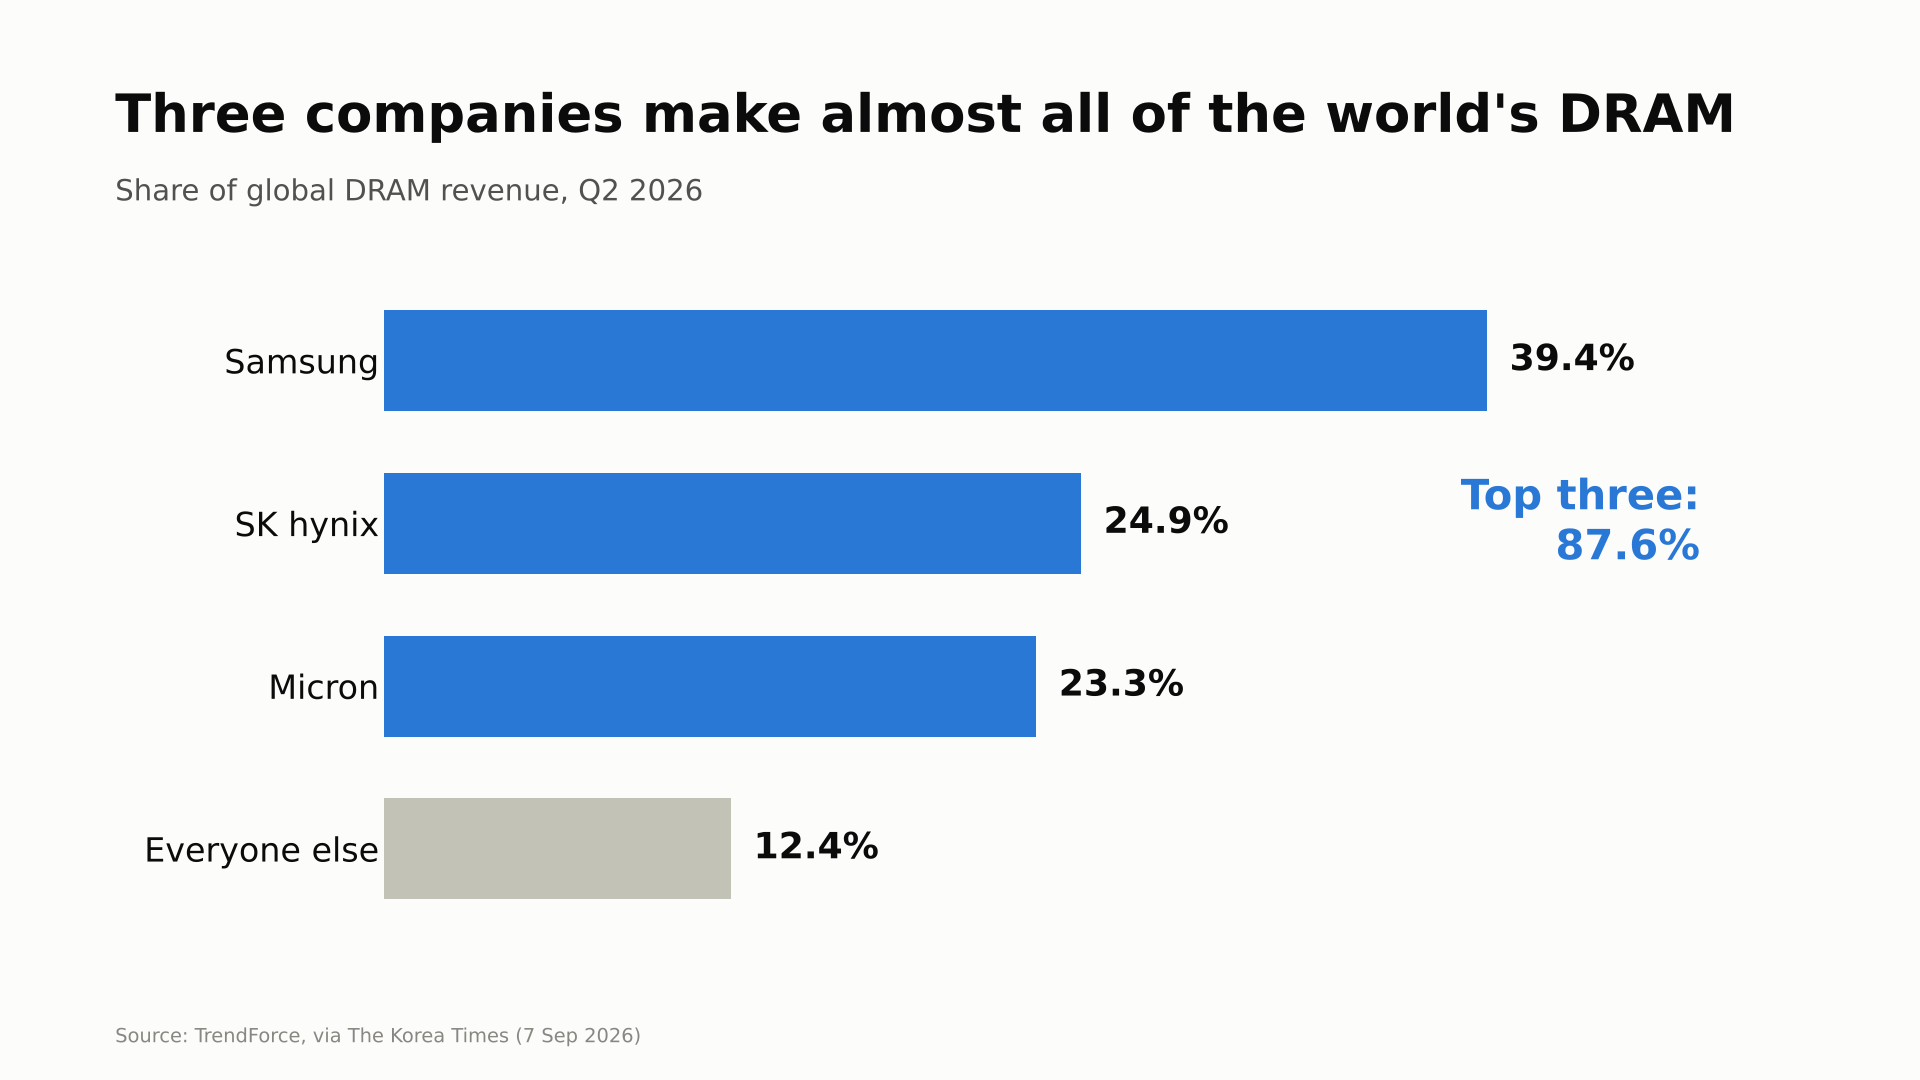
\includegraphics[width=0.85\linewidth]{figures/02_market_share.png}
  \caption{Global DRAM revenue share, Q2 2026. Source: TrendForce via The Korea Times \cite{koreatimes}.}
  \label{fig:share}
\end{figure}

There are two main kinds of memory chip:
\begin{itemize}
  \item \textbf{DRAM} is working memory: the RAM in PCs and phones, and the memory in servers.
  \item \textbf{NAND flash} is storage: the chips inside SSDs, phones and memory cards.
\end{itemize}

AI accelerators use a special, stacked form of DRAM called \textbf{HBM} (high-bandwidth memory). HBM sells at much higher margins than ordinary RAM, but it uses up advanced wafer and packaging capacity that could otherwise make conventional chips.

Memory is also famously cyclical. The last bust was only three years ago: in late 2022, DRAM and NAND prices roughly halved, and Micron cut about 10\% of its staff \cite{dcd}. Today's shortage is the upswing of the same cycle, pushed much harder by AI. Sections~\ref{sec:cycle} and~\ref{sec:wins} show both halves of that cycle in the data.

\section{Data and method}

The project combines three time-series datasets we compiled from public sources with figures reported by analysts. The datasets are provided as CSV files alongside this report (\texttt{data/}).

\begin{table}[h]
  \centering\small
  \begin{tabularx}{\linewidth}{@{}p{3.6cm}Xp{3.4cm}@{}}
    \toprule
    \textbf{Dataset} & \textbf{What it contains} & \textbf{Source} \\
    \midrule
    DDR4 contract price & Monthly average contract price of a DDR4 8Gb DRAM chip, 18 reported months from Jan 2022 to Sep 2026 & DRAMeXchange, as compiled by Silicon Analysts \cite{silicon} \\
    \addlinespace
    Hyperscaler capex & Quarterly capital expenditure of Microsoft, Amazon, Alphabet, Meta and Oracle, Q1 2022 to Q4 2025 & Epoch AI, from company SEC filings \cite{epoch} \\
    \addlinespace
    SK hynix operating profit & Quarterly operating profit or loss, 4Q22 to 2Q26 & SK hynix results releases \cite{skhynix} \\
    \bottomrule
  \end{tabularx}
  \caption{Datasets compiled for this project.}
  \label{tab:data}
\end{table}

We cleaned and reconciled each series. Capex company totals were checked against the reported total, and one missing SK hynix quarter (2Q23) was confirmed from a later release. Each chart was then chosen for the question it answers: line charts for price trends over time, stacked bars for parts of a total over time, and bars about zero for gains and losses. A consistent, colourblind-safe palette is used throughout, and every chart is also produced as an animated clip for the accompanying video.

\section{Why prices rose}

Prices rose because AI demand pulled memory supply away from everyone else, and supply could not grow fast enough to make up the gap. There are four links in the chain:

\begin{enumerate}
  \item \textbf{AI spending exploded.} Major cloud providers' combined capex is projected to rise 98\% in 2026. DRAM and NAND are expected to take 47\% of that spend \cite{infotech}.
  \item \textbf{Makers moved capacity to where the margin is.} HBM and server DRAM are expected to take 51\% of all DRAM bit supply in 2026. Ordinary PC and phone memory gets what is left.
  \item \textbf{Cloud giants locked in supply.} Large providers signed long-term agreements and accept higher prices to guarantee supply. Some PC makers and module makers now receive reduced allocations \cite{trendforce}.
  \item \textbf{SSDs followed.} AI also needs fast storage, so enterprise SSDs absorbed NAND flash. Consumer SSD supply is being held back to protect prices, and phone storage (eMMC/UFS) shares capacity with higher-margin enterprise drives.
\end{enumerate}

The key point is that weaker PC or phone sales cannot fix this. The demand driving the shortage comes from data centres, not consumers.

\subsection*{The demand, in data}

Figure~\ref{fig:capexq} shows link 1 directly. In Q1 2022, the five largest cloud spenders together invested \$37.6 billion a quarter. By Q4 2025 it was \$140.6 billion, 3.7$\times$ as much, with the steepest rise from 2024 onwards \cite{epoch}.

\begin{figure}[!htbp]
  \centering
  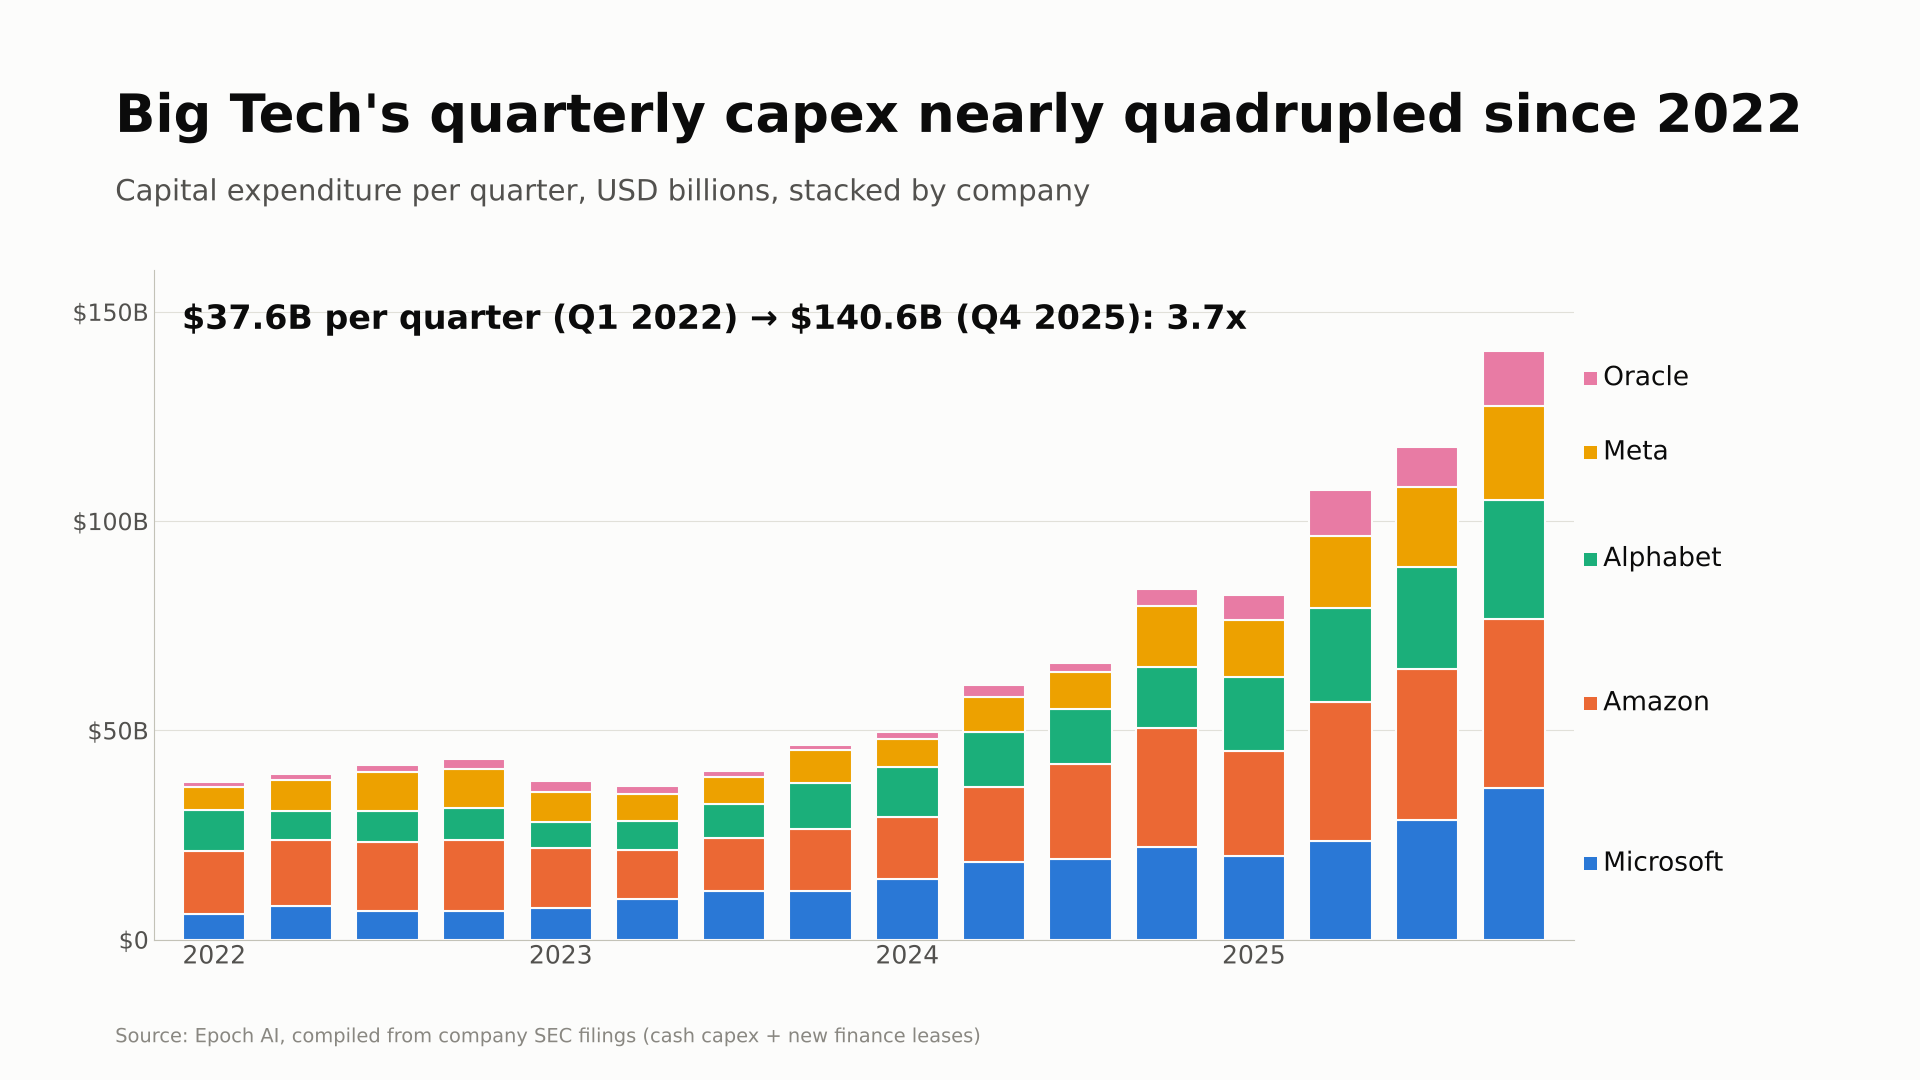
\includegraphics[width=0.95\linewidth]{figures/04_capex_quarterly.png}
  \caption{Quarterly capital expenditure of five hyperscalers, stacked by company. Source: Epoch AI, from SEC filings \cite{epoch}.}
  \label{fig:capexq}
\end{figure}

\section{How big the increase is}\label{sec:cycle}

The clearest view of the cycle is the contract price of a single memory chip over time (Figure~\ref{fig:cycle}). A DDR4 8Gb chip fell 62\%, from \$3.41 in January 2022 to \$1.30 in August 2023, during the post-pandemic bust. From mid-2025 the price climbed almost vertically, reaching \$26 in September 2026: 20$\times$ its 2023 low \cite{silicon}. DDR4 overstates the general rise, because all three makers announced in 2025 that they were phasing DDR4 out, which squeezed its supply further \cite{ddr4eol}. But newer memory moved the same way, as the retail and contract figures below show.

\begin{figure}[!htbp]
  \centering
  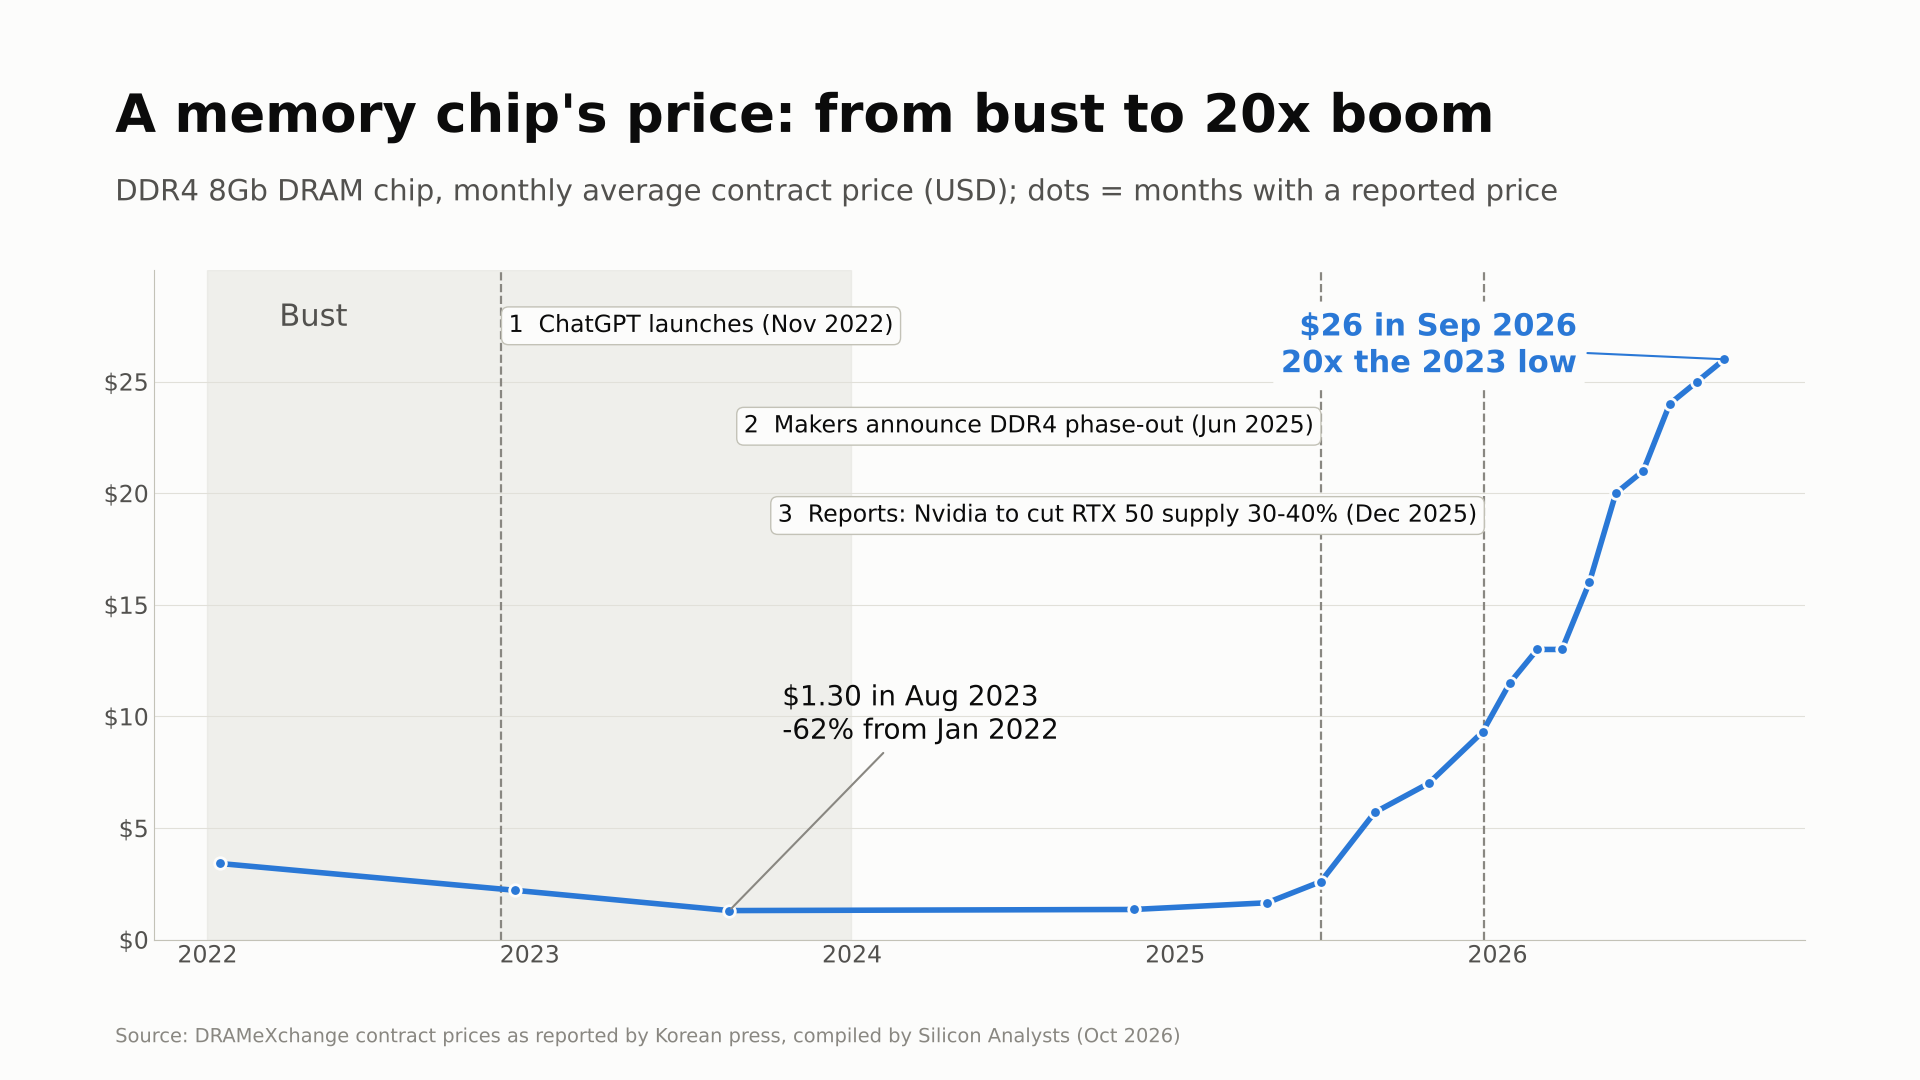
\includegraphics[width=0.95\linewidth]{figures/05_dram_price_cycle.png}
  \caption{DDR4 8Gb DRAM chip, monthly average contract price; dots mark months with a reported price. Source: DRAMeXchange via Silicon Analysts \cite{silicon}.}
  \label{fig:cycle}
\end{figure}

At retail, a 2$\times$16GB DDR5-4800 kit went from about \$90 in August 2025 to \$425 in August 2026, roughly 4.7$\times$ (Figure~\ref{fig:kit}).

\begin{figure}[!htbp]
  \centering
  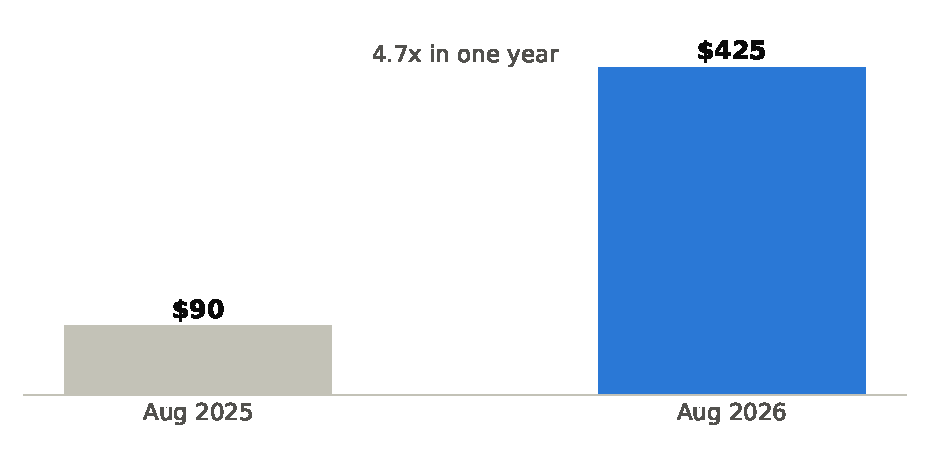
\includegraphics[width=0.72\linewidth]{figures/ram_kit.pdf}
  \caption{A 32GB (2$\times$16GB) DDR5-4800 RAM kit, US retail price, one year apart. Source: Tom's Hardware prices compiled by Tech-Insider \cite{techinsider}.}
  \label{fig:kit}
\end{figure}

Retail prices vary by store and region, so contract prices (what PC makers pay) are the more reliable measure (Table~\ref{tab:prices}).

\begin{table}[h]
  \centering\small
  \begin{tabularx}{\linewidth}{@{}Xlll@{}}
    \toprule
    \textbf{Product} & \textbf{Price change} & \textbf{Period} & \textbf{Source} \\
    \midrule
    Conventional DRAM (contract) & +58--63\% & One quarter, Q2 2026 & TrendForce \cite{trendforce} \\
    NAND flash (contract) & +70--75\% & One quarter, Q2 2026 & TrendForce \cite{trendforce} \\
    Server DRAM & $\sim$+270\% (forecast) & Across 2026 & TrendForce \cite{infotech} \\
    Enterprise SSD & $\sim$+235\% (forecast) & Across 2026 & TrendForce \cite{infotech} \\
    DRAM + SSD combined & +130\% (forecast) & By end of 2026 & Gartner \cite{gartner} \\
    \bottomrule
  \end{tabularx}
  \caption{Memory price changes, contract and forecast.}
  \label{tab:prices}
\end{table}

Suppliers are earning record revenue as a result. Global DRAM revenue rose 59.5\% in one quarter to \$154.7 billion in Q2 2026 \cite{koreatimes}.

Not every price is rising. In late September 2026, NAND wafer spot prices slipped about 1\% as consumer demand weakened, so storage may ease before RAM does \cite{infotech}.

\section{Who feels it}

The cost lands hardest on consumer devices, where memory is a growing share of what a product costs to build (Figure~\ref{fig:impact}).

\begin{figure}[!htbp]
  \centering
  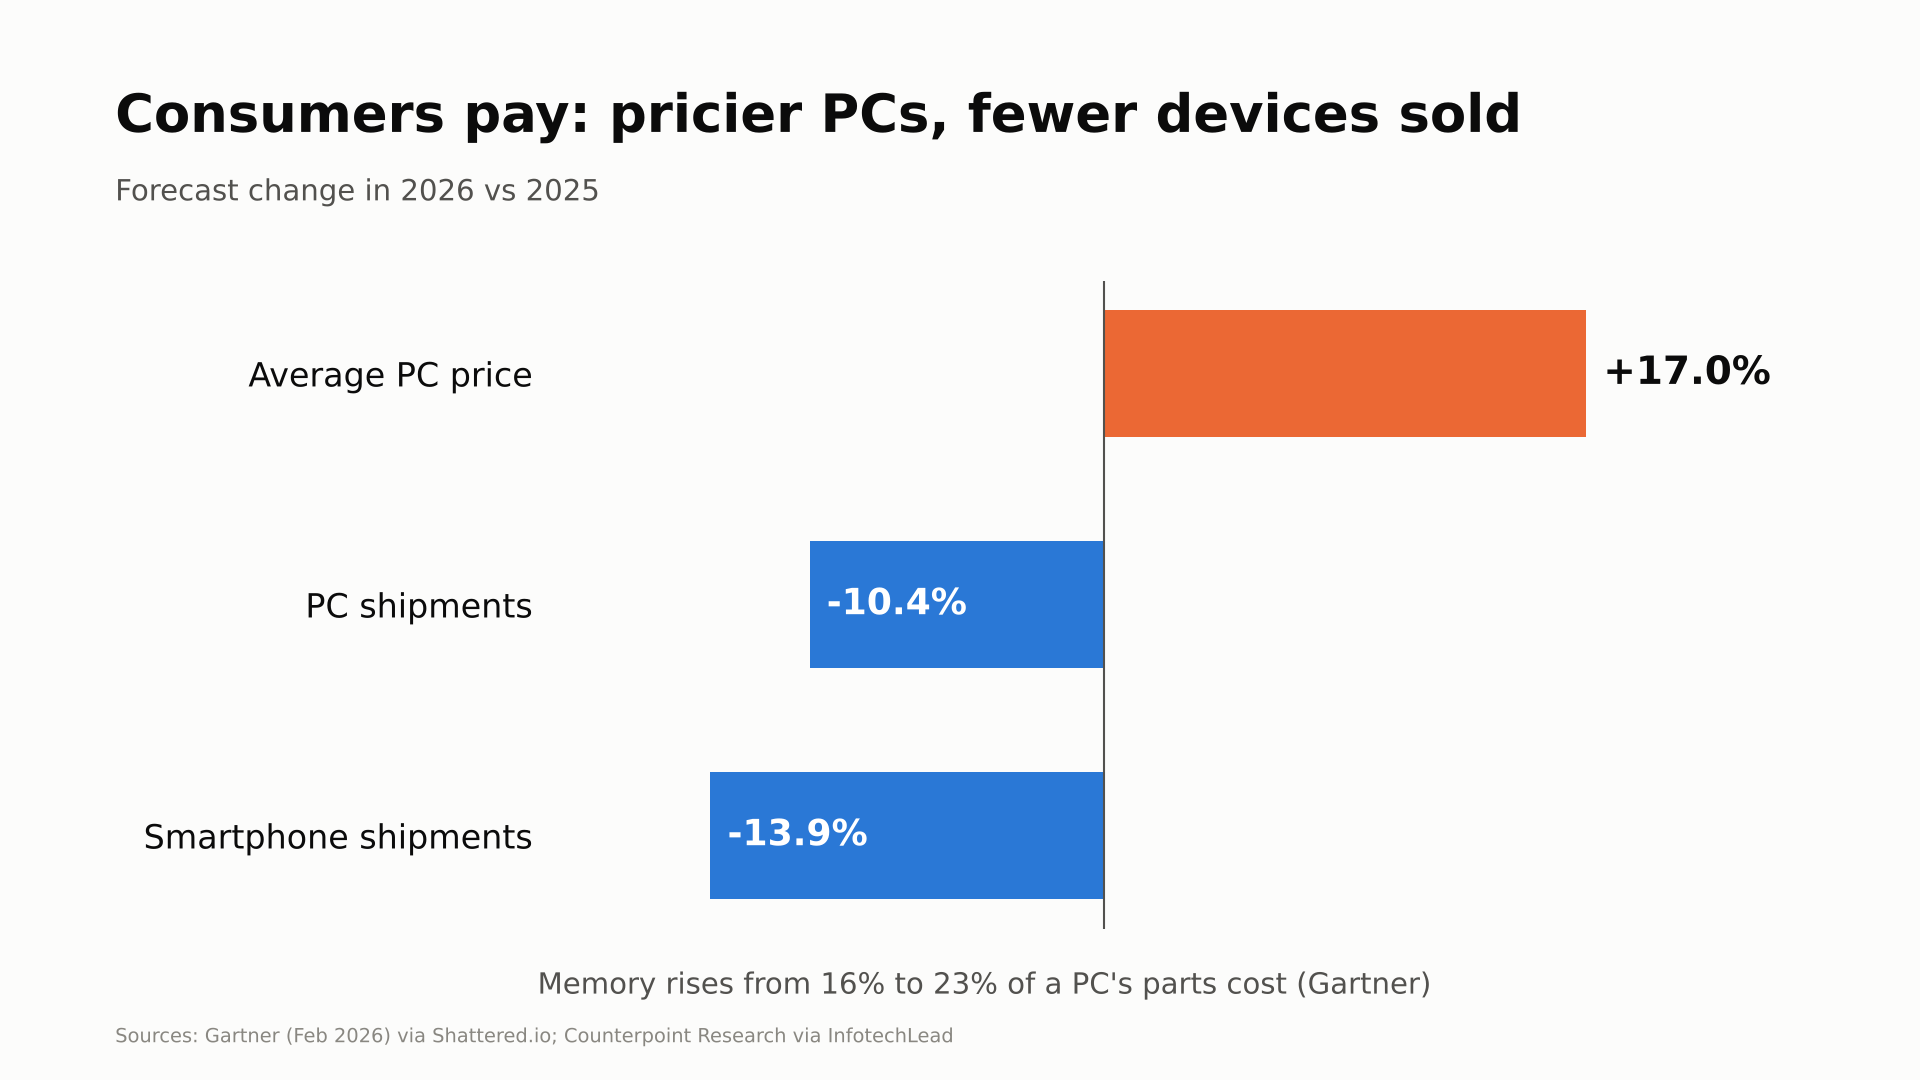
\includegraphics[width=0.85\linewidth]{figures/06_consumer_impact.png}
  \caption{Forecast change in 2026 vs 2025. Sources: Gartner \cite{gartner}; Counterpoint Research via InfotechLead \cite{infotech}.}
  \label{fig:impact}
\end{figure}

\begin{itemize}
  \item \textbf{PCs:} Gartner expects average PC prices to rise 17\% in 2026 and shipments to fall 10.4\%. Memory rises from 16\% to 23\% of a PC's bill of materials \cite{gartner}.
  \item \textbf{Smartphones:} memory can be close to 60\% of the parts cost of a phone priced around \$400. Counterpoint Research expects 2026 smartphone shipments to fall 13.9\% to about 1.08 billion units \cite{infotech}.
  \item \textbf{DIY builders and students:} retail RAM kits roughly quadrupled within a year, so upgrades and new builds cost far more than planned.
  \item \textbf{Smaller manufacturers:} they have less buying power than the big PC and phone brands, and struggle to secure supply at any price.
\end{itemize}

Device makers have four options: absorb the cost, raise prices, ship less memory as standard, or delay launches. The first squeezes their margins, and the other three pass the cost on to buyers.

\section{Who wins: the memory makers}\label{sec:wins}

The same shortage that raises device prices has transformed memory makers' profits. SK hynix made operating losses for four straight quarters, from 4Q22 to 3Q23, with its worst operating loss of 3.4 trillion won in 1Q23. In 2Q26 it earned 60.5 trillion won, at a 76\% operating margin (Figure~\ref{fig:hynix}) \cite{skhynix}.

\begin{figure}[!htbp]
  \centering
  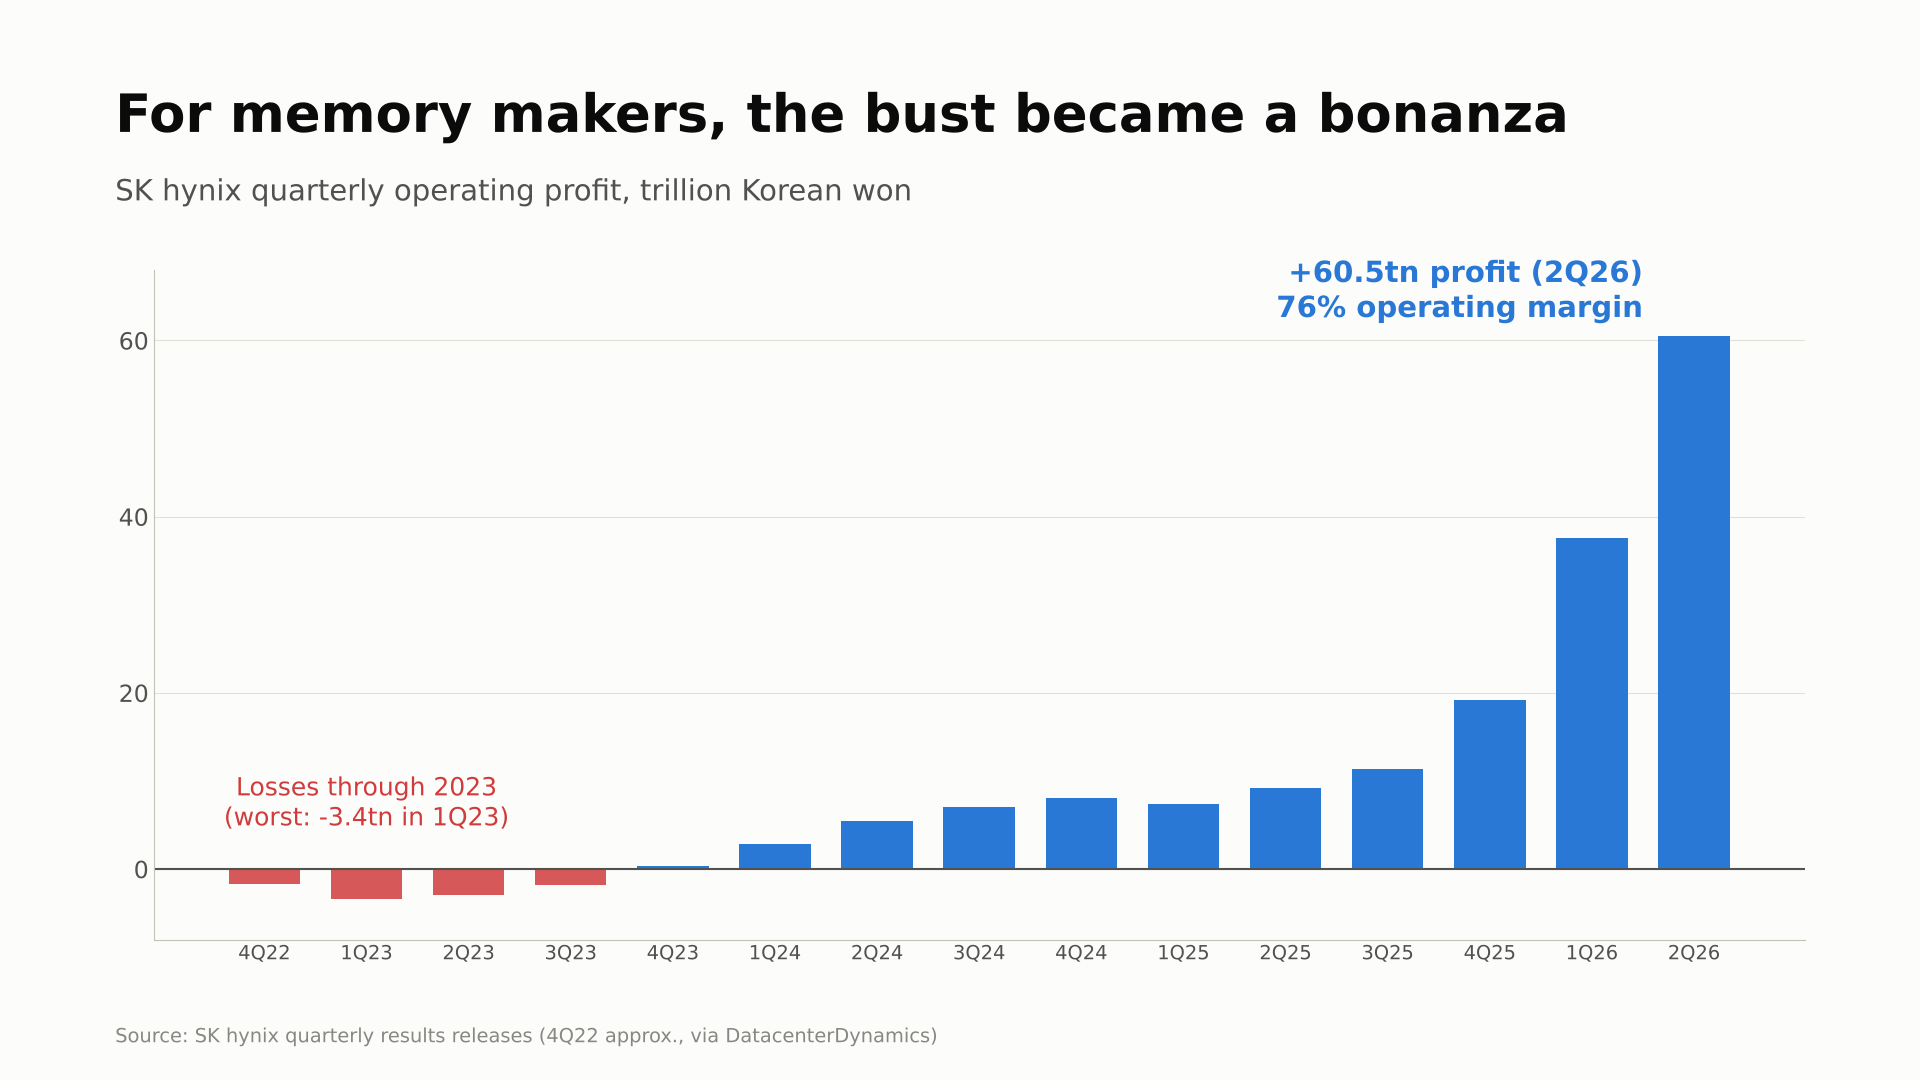
\includegraphics[width=0.95\linewidth]{figures/07_skhynix_profit.png}
  \caption{SK hynix quarterly operating profit, trillion won. 4Q22 is approximate. Source: company results releases \cite{skhynix}, DatacenterDynamics \cite{dcd}.}
  \label{fig:hynix}
\end{figure}

\section{When it might ease}

Not before 2027 for DRAM, on current forecasts. New capacity is coming, but it takes a year or more to build, qualify and ramp up \cite{infotech}.

\begin{itemize}
  \item \textbf{More supply in 2027:} new fabs and process upgrades should lift combined server DRAM and HBM supply by about 27\% in 2027 (TrendForce).
  \item \textbf{A warning from SK hynix:} the company has said 2027 could be the industry's tightest year yet for supply capacity.
  \item \textbf{A new competitor:} China's CXMT began mass production of a newer DRAM generation in September 2026 and raised \$8.6 billion in its 2026 IPO. Its chips still need time to qualify with customers.
  \item \textbf{NAND may balance first:} with consumer demand weak, storage could rebalance before RAM does.
\end{itemize}

The biggest swing factor is not on this list: it is whether AI spending keeps growing, which the next two sections examine.

\section{Is AI a bubble? The case that it is}

A bubble is spending or prices running far ahead of the value that eventually shows up. The worry here is the sheer size of the build-out (Figure~\ref{fig:capex}).

\begin{figure}[!htbp]
  \centering
  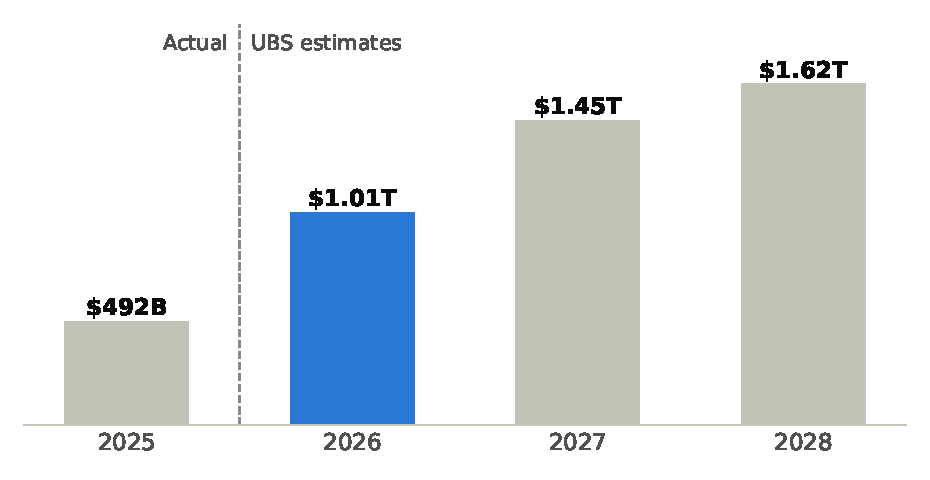
\includegraphics[width=0.78\linewidth]{figures/capex.pdf}
  \caption{Big Tech capex doubles to about \$1 trillion in 2026. Hyperscaler capital expenditure, USD; 2026--2028 are UBS estimates. Source: 24/7 Wall St. via Yahoo Finance \cite{ubs}.}
  \label{fig:capex}
\end{figure}

Skeptics point to four warning signs:

\begin{itemize}
  \item \textbf{Spending matches revenue.} Amazon, Alphabet and Microsoft are spending about 102\% of their cloud revenue on capex in 2026 \cite{ubs}.
  \item \textbf{A depreciation bill is coming.} AI chips are written off over about six years. Morgan Stanley estimates up to 40\% of this year's AI capex won't be running until 2027--29, and annual depreciation could reach \$500 billion to \$1 trillion by 2030 \cite{benzinga}.
  \item \textbf{Debt is creeping in.} Hyperscalers issued about \$225 billion in bonds this year. Morgan Stanley forecasts about \$550 billion of negative free cash flow next year \cite{benzinga}.
  \item \textbf{Profits may be flattered.} Paper gains on stakes in private AI labs added about \$222 billion to the big four's earnings over the four quarters to mid-2026 \cite{benzinga}.
\end{itemize}

\section{The case that it isn't, and a middle view}

The strongest counter-argument is that today's leaders look nothing like the companies at the 2000 dot-com peak (Figure~\ref{fig:val}). IoT Analytics makes four points \cite{iot}:

\begin{figure}[!htbp]
  \centering
  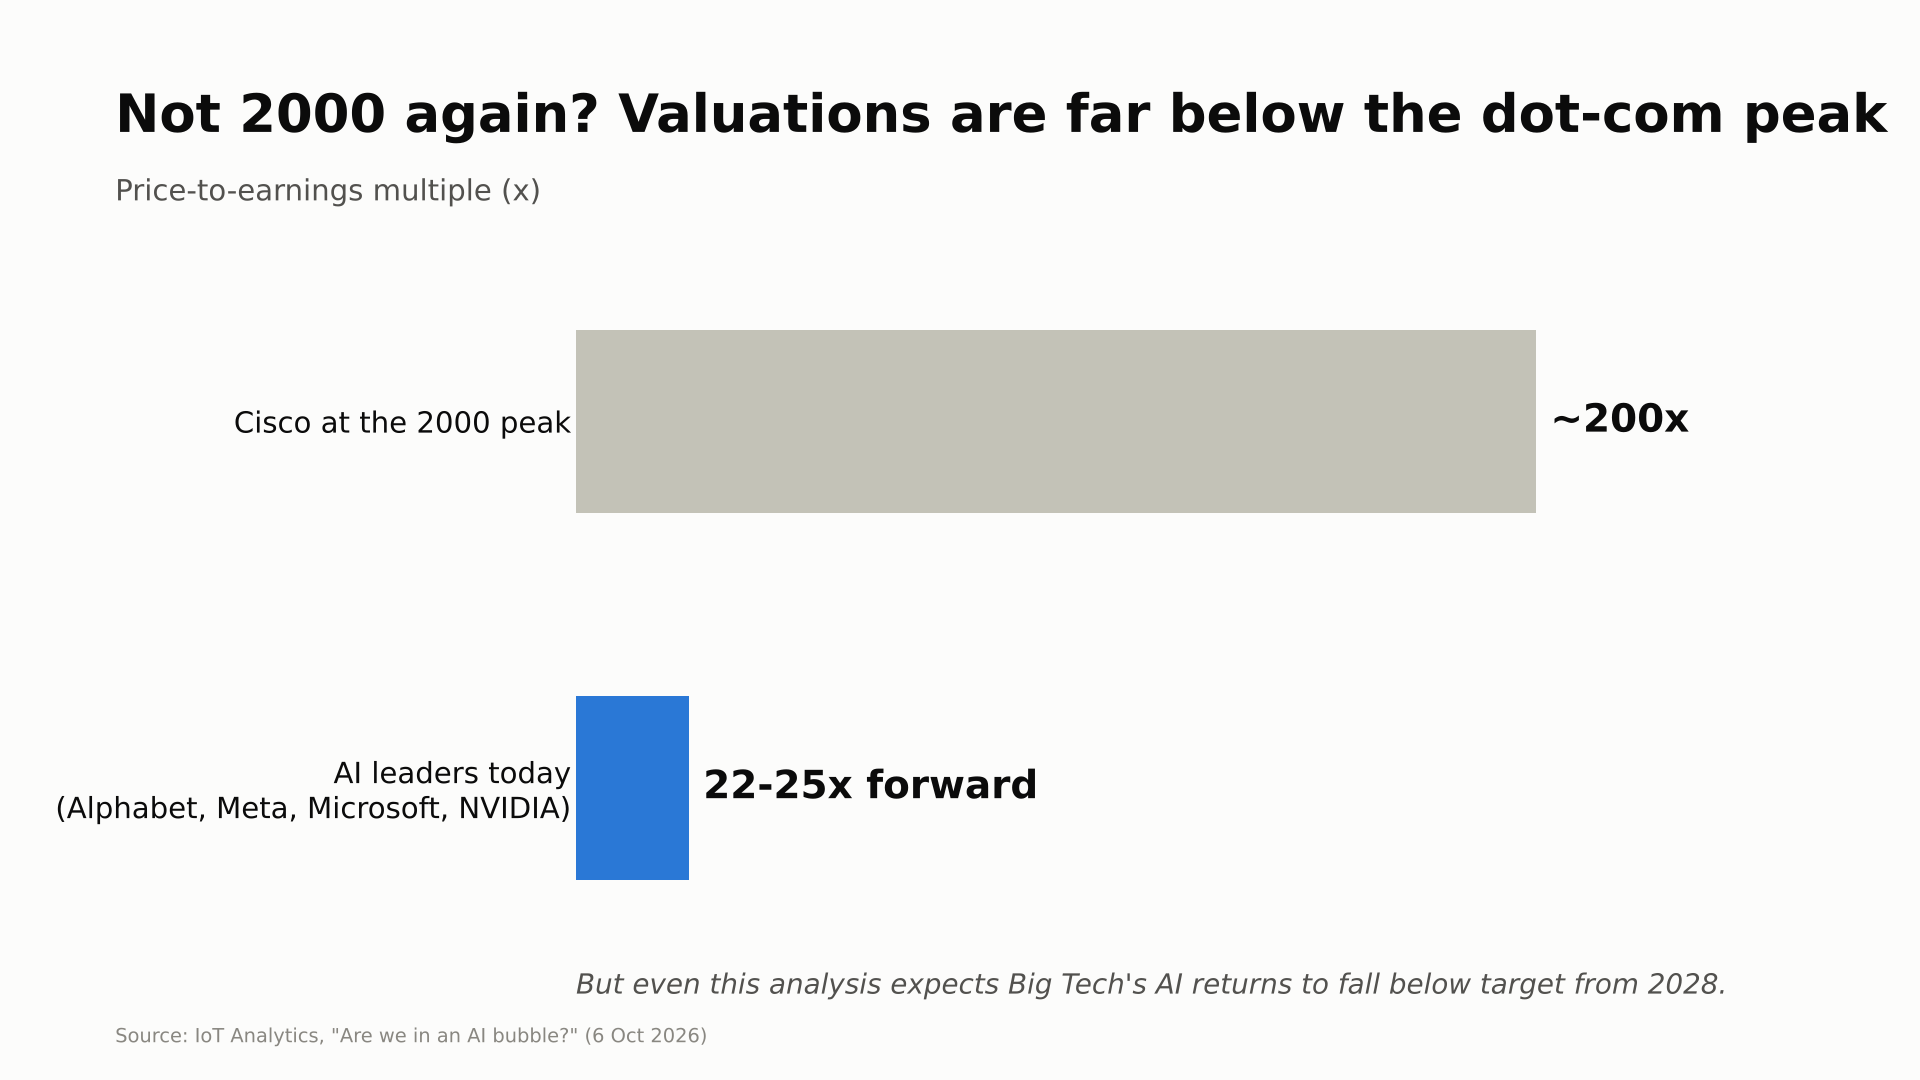
\includegraphics[width=0.85\linewidth]{figures/09_valuations.png}
  \caption{Price-to-earnings multiples: Cisco at the 2000 peak vs today's AI leaders (forward). Source: IoT Analytics \cite{iot}.}
  \label{fig:val}
\end{figure}

\begin{itemize}
  \item \textbf{Valuations are not extreme.} Alphabet, Meta, Microsoft and NVIDIA trade at about 22--25$\times$ forward earnings, against about 200$\times$ for Cisco in 2000.
  \item \textbf{Demand is real and growing.} Generative AI spending roughly doubled to \$308 billion in 2025. CoreWeave's contracted backlog rose from \$15 billion to \$66.8 billion in a year.
  \item \textbf{The spenders can afford it.} Most of the build-out is paid from operating cash flow by companies with other profitable businesses. That is unlike the debt-funded telecom build-out of 2000.
  \item \textbf{Cheaper AI means more use.} Token prices fell over 90\% in three years, which tends to raise total consumption.
\end{itemize}

Even this ``no bubble'' analysis projects hyperscaler returns falling below their 15\% target from 2028. So the two sides agree on more than their labels suggest.

\begin{accentbox}
\textbf{Middle view.} AI is a real technology with real demand, but the infrastructure is likely being built faster than revenue can justify for a few years. The realistic downside is large write-downs, weaker profits and a spending slowdown, mostly absorbed by cash-rich giants. A collapse is less likely, though debt-heavy smaller cloud providers are more exposed.
\end{accentbox}

\section{How the two connect}

Memory prices are a downstream bet on AI spending. Data centres are the source of the demand, so the path of AI capex largely decides the path of RAM and SSD prices. The three scenarios in Table~\ref{tab:scen} are our reasoning from the evidence above, not forecasts from a source.

\begin{table}[h]
  \centering\small
  \begin{tabularx}{\linewidth}{@{}>{\bfseries}p{2.6cm}XX@{}}
    \toprule
    \textnormal{\textbf{Scenario}} & \textbf{What happens to AI spending} & \textbf{What happens to memory prices} \\
    \midrule
    Boom continues & Capex keeps rising toward UBS's \$1.45 trillion for 2027 & DRAM stays tight through 2027. Consumer RAM stays expensive; SSDs may ease a little sooner. \\
    \addlinespace
    Slowdown & Growth in capex flattens as returns disappoint & New fabs come online into softer demand. Prices drift down through 2027--28. \\
    \addlinespace
    Bubble deflates & Data-centre orders are cut sharply & Memory has a long boom-bust record (prices roughly halved in 2022). A fast price fall becomes likely. \\
    \bottomrule
  \end{tabularx}
  \caption{Scenarios linking AI spending to memory prices.}
  \label{tab:scen}
\end{table}

The irony is that the supply being built to meet AI demand would turn into a glut if that demand faded. That is how the 2022 bust happened, on a smaller scale.

\section{Conclusion and what to watch}

The memory price surge is the most visible everyday sign of the AI boom. It will last as long as AI spending keeps growing, and on current guidance that means DRAM stays expensive into 2027. If the bubble skeptics are right, the reversal could be just as sharp.

Four signals show which way it is going:
\begin{itemize}
  \item \textbf{Hyperscaler capex guidance} in each quarter's earnings calls (Alphabet, Amazon, Meta, Microsoft). Cuts here come before memory prices fall.
  \item \textbf{TrendForce's quarterly contract price forecasts.} The first forecast of flat or falling DRAM prices marks the turn.
  \item \textbf{Retail RAM and SSD prices.} NAND spot prices are already softening, so SSDs may turn first.
  \item \textbf{New supply.} Watch whether the expected 2027 capacity, including CXMT's, reaches customers on schedule.
\end{itemize}

{\small\color{muted} This report uses forecasts and estimates that may be revised. It is not investment advice.}

\begingroup\raggedright
\begin{thebibliography}{99}\small
\bibitem{trendforce} TrendForce, ``AI Server Demand to Drive Memory Contract Price Increases in 2Q26,'' 31 Mar 2026. \url{https://www.trendforce.com/presscenter/news/20260331-12995.html}
\bibitem{infotech} InfotechLead, ``Why Are Memory Prices Rising in 2026?'' (citing TrendForce, Reuters, Counterpoint). \url{https://infotechlead.com/data-center/why-are-memory-prices-rising-in-2026-ai-boom-tightens-dram-hbm-and-nand-supply-98428}
\bibitem{koreatimes} The Korea Times, Samsung's DRAM market share report (citing TrendForce), 7 Sep 2026. \url{https://www.koreatimes.co.kr/business/20260907/samsung-extends-lead-in-global-dram-market-with-39-share-report}
\bibitem{gartner} Shattered.io, ``Memory Chip Shortage 2026: PC Prices Up 17\%, Gartner Says'' (citing Gartner, 26 Feb 2026). \url{https://shattered.io/memory-chip-shortage-pc-prices-up-17-percent-2026/}
\bibitem{techinsider} Tech-Insider, ``DDR5 RAM Prices Up 110\% as AI Devours Memory'' (citing Tom's Hardware). \url{https://tech-insider.org/ddr5-ram-prices-2026/}
\bibitem{dcd} DatacenterDynamics, ``SK Hynix posts first loss in 10 years as memory market struggles,'' 1 Feb 2023. \url{https://www.datacenterdynamics.com/en/news/sk-hynix-posts-first-loss-in-10-years-as-memory-market-struggles}
\bibitem{ubs} 24/7 Wall St. via Yahoo Finance, ``Hyperscalers Are Spending 102\% of Cloud Revenue on Capex'' (UBS estimates), 22 Aug 2026. \url{https://finance.yahoo.com/technology/ai/articles/ai-absurd-spending-boom-hyperscalers-162709082.html}
\bibitem{benzinga} Benzinga, ``A \$1 Trillion Depreciation Bomb Is Ticking Beneath the AI Market'' (citing Morgan Stanley, BCA Research), 25 Oct 2026. \url{https://www.benzinga.com/markets/tech/26/10/62580225/a-1-trillion-depreciation-bomb-is-ticking-beneath-the-ai-market}
\bibitem{iot} IoT Analytics, ``Are we in an AI bubble?'' 6 Oct 2026. \url{https://iot-analytics.com/why-there-is-no-ai-bubble-analysis/}
\bibitem{silicon} Silicon Analysts, ``DRAM Spot \& Contract Price (DDR4 8Gb),'' compiling DRAMeXchange monthly contract prices, accessed 26 Oct 2026. \url{https://siliconanalysts.com/market-data/dram-ddr4-price}
\bibitem{epoch} Epoch AI, ``Hyperscaler capex has quadrupled since GPT-4's release,'' 26 Feb 2026, data from company SEC filings. \url{https://epoch.ai/data-insights/hyperscaler-capex-trend}
\bibitem{skhynix} SK hynix, quarterly financial results releases (1Q23, 4Q23, 2Q24, 4Q24, 3Q25, 1Q26, 2Q26). \url{https://news.skhynix.com/en/q2-2026-business-results/}
\bibitem{ddr4eol} TrendForce, ``DDR4 Exit Timeline Unfolds for Top Memory Makers,'' 9 Jul 2025. \url{https://www.trendforce.com/news/2025/07/09/news-ddr4-exit-timeline-unfolds-for-top-memory-makers-plans-for-samsung-sk-hynix-and-micron}
\end{thebibliography}
\endgroup

\end{document}
